%%%%%%%%%%%%%%%%%%%%%%%%%%%%%%%%%%%%%%%%%%%%%%%%%%%%%%%%%%%%%%%%%%%%%%%%%%%%%%%%
%2345678901234567890123456789012345678901234567890123456789012345678901234567890
%        1         2         3         4         5         6         7         8

%\documentclass[letterpaper, 10 pt, conference]{ieeeconf}  % Comment this line out if you need a4paper

\documentclass[a4paper, 10pt, conference]{ieeeconf}      % Use this line for a4 paper

%\IEEEoverridecommandlockouts                              % This command is only needed if
                                                          % you want to use the \thanks command

\overrideIEEEmargins                                      % Needed to meet printer requirements.

% See the \addtolength command later in the file to balance the column lengths
% on the last page of the document

% The following packages can be found on http:\\www.ctan.org
\usepackage{graphics} % for pdf, bitmapped graphics files
%\graphicspath{{../images/}}
\usepackage{epsfig} % for postscript graphics files
\usepackage{mathptmx} % assumes new font selection scheme installed
\usepackage{times} % assumes new font selection scheme installed
\usepackage{amsmath} % assumes amsmath package installed
\usepackage{amssymb}  % assumes amsmath package installed
\usepackage{epstopdf}
\usepackage{color}
\definecolor{tumblue}{rgb}{0, 0.4, 0.74}

\title{\LARGE \bf
Controlling an Ophthalmic Surgery Robot with Matlab \& Simulink
}
%the original title below wasnt really appropriate any more I think...
%Preparation of Papers for Robot-assisted Surgery in Clinics*


%\author{Various Authors% <-this % stops a space
%\\Technische Universit\"at M\"unchen\\
%Email: also various}
%commented this out because our names etc are already on the title page


\begin{document}

\begin{figure*}[!h]

  
\includegraphics{./images/knoll-blue.pdf}  
\includegraphics{./images/IN.pdf} \hfill 
\includegraphics{./images/tumlogo.pdf}

  \vspace*{1cm}
  {\large \textsf{Robotics and Embedded Systems}}\\
  {\large \textsf{Department of Informatics}}\\
  {\large \textsf{Technische Universit{\"a}t M{\"u}nchen}}\\




  \vspace*{5cm}
%
%
% TITEL DER ARBEIT
%
%
  {\color{tumblue} \Huge \bf \textsf{Controlling an Ophthalmic Surgery Robot with Matlab \& Simulink}}\\  % HIER EINSETZEN!

  \vspace*{1cm}
%
%
% NAME DES STUDENTEN (auf Titelblatt)
%
%

  \begin{tabular}{l c l}
  	\Large \bf \textsf{Gheorghita, Daniel} & \Large \bf \textsf{MatNr.} & \Large \bf \textsf{daniel0392@gmail.com}\\
  	\Large \bf \textsf{Paulis, Bogdan} & \Large \bf \textsf{MatNr.} & \Large \bf \textsf{bogdan\_ paulis@yahoo.com}\\
  	\Large \bf \textsf{Swazinna, Phillip} & \Large \bf \textsf{03686497} & \Large \bf \textsf{p.swazinn@atum.de}\\
  	\Large \bf \textsf{L\" ohr, Timo} & \Large \bf \textsf{MatNr.} & \Large \bf \textsf{timo.loehr@tum.de}\\
  	\Large \bf \textsf{Deutrich, Matthias} & \Large \bf \textsf{MatNr.} & \Large \bf \textsf{matthias-deutrich@t-online.de}\\
  	\Large \bf \textsf{Neves, Miguel} & \Large \bf \textsf{MatNr.} & \Large \bf \textsf{chukas.spam@gmail.com}
  \end{tabular}
 % HIER EINSETZEN!

  \vspace*{5cm}
  {\Large \textsf{Seminar \emph{Robot-assisted Surgery in Clinics} SS 2017}}\\

  \vspace*{1cm}
  \begin{tabular}{ll}
%
%
% NAME DES BETREUERS
%
%
    {\Large \bf \textsf{Advisor:}} &
    {\Large \textsf{Mingchuan Zhou}}\\                  % HIER EINSETZEN!
    \\

    {\Large \bf \textsf{Supervisor:}} &
    {\Large \textsf{Prof. Dr.-Ing. Alois Knoll}}\\
    \\

%
%
% ABGABETERMIN
%
%
    {\Large \bf \textsf{Submission:}} &
    {\Large \textsf{17. July 2017}}

  \end{tabular}

\end{figure*}


\maketitle
\thispagestyle{empty}
\pagestyle{empty}

\begin{abstract}
this is the content of the abstract file
\end{abstract}

\section{INTRODUCTION}
this is the content of the introduction file

\section{Connecting VREP with Matlab (Daniel)}
this is the content of Daniel\rq s file

\section{Inverse Kinematics (Bogdan)}
this is the content of Bogdan\rq s file

\section{Simulink GUI for Control (Phillip)}
Given that it was our task to control the robot with matlab, simulink was deemed to be the perfect tool to create a small GUI for this project.\\
As we were required to be able to draw different shapes, this GUI contains a switch, which enables the user to choose from a heart, square, or circle shape. Additionally, there are three sliders corresponding to the X, Y, and Z axes, in case users would like to take matters into their own hands. See the figure below for reference.\\
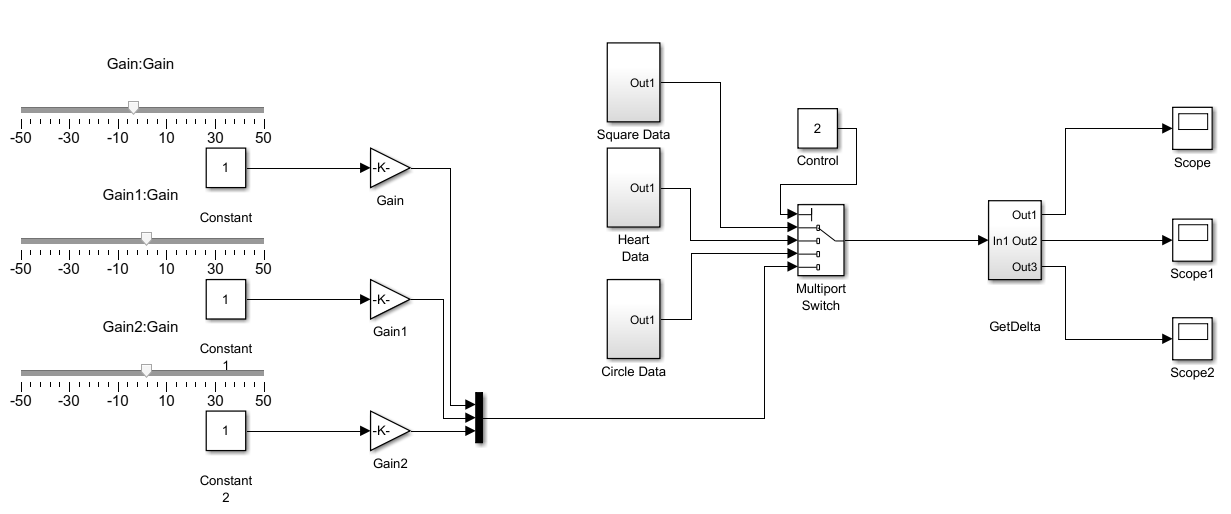
\includegraphics[scale=.4]{images/simulink_gui.png}

\section{Creation of Shapes (Timo)}
this is the content of Timo\rq s file

\section{Getting the needle to the entry point of the eye (Matthias)}
I hope this is what you were doing, I wasn\rq t quite sure any more, because it wasn\rq t listed in the ToDo...\\
this is the content of Matthias\rq file
\section{Different Algorithm for Robot control (Miguel)}
Same as Matthias ;)\\
this is the content of Miguel\rq s file

\section*{Abbreviations and Acronyms}
Define abbreviations and acronyms - not sure if we need this?

\addtolength{\textheight}{-12cm} 
% This command serves to balance the column lengths
% on the last page of the document manually. It shortens
% the textheight of the last page by a suitable amount.
% This command does not take effect until the next page
% so it should come on the page before the last. Make
% sure that you do not shorten the textheight too much.

\section*{APPENDIX}

Appendixes should appear before the acknowledgment - keeping this section for god knows what...

\section*{ACKNOWLEDGMENT}

Same...

I put the Master\rq s Thesis in the bibliography, wasn\rq t sure whether we needed anything else - maybe the Algorithm (that I  think) Miguel worked on.
\begin{thebibliography}{99}
\bibitem{c1} P. Gschirr, Control and Simulation of a Robotic Setup for Assisting Ophthalmic Surgery, Master Thesis at the Computer Science Department of the Technical University of Munich. Munich: 2014
\end{thebibliography}

\end{document}